%%%%%%%%%%%%%%%%%%%%%%%%%%%%%%%%%%%%%%%%%%%%%%%%%%%%
\documentclass[a4paper,fleqn,10pt]{SICE_ISCS}
%\usepackage{url}
\usepackage{ascmac}
\usepackage{amssymb}
%\usepackage{amsmath}
%\usepackage{hyperref}
%\usepackage{lmodern}
\usepackage{breqn}
\usepackage{bm}
\usepackage{comment}
\usepackage{pdfpages}
\usepackage{algorithm}
\usepackage{algorithmic}

\makeatletter
\@ifundefined{theorem}{%
  \newtheorem{theorem}{Theorem}
}{}
\@ifundefined{definition}{%
  \newtheorem{definition}{Definition}
}{}
\makeatother

%\usepackage{HERE}
%\usepackage[version=3]{mhchem}%%化学式
%\usepackage{siunitx}
% Packages for Japanese language support
%\usepackage{CJKutf8}
%\usepackage{otf}
\usepackage[dvipdfmx]{hyperref}
%\usepackage{pxjahyper}
\usepackage{cite}
\usepackage{ulem} % Package for strikethrough
\usepackage{caption}
\captionsetup{font=small} % キャプションのフォントサイズを小さく設定
\usepackage{float} % figureの位置を固定するためのパッケージ
\DeclareGraphicsExtensions{.eps,.pdf,.png,.jpg}
\newcommand{\Tabref}[1]{{Table~\ref{#1}}}
\newcommand{\Eqref}[1]{式~(\ref{#1})}
\newcommand{\Figref}[1]{{Fig.~\ref{#1}}}
\newcommand{\blue}[1]{\textcolor{blue}{#1}}
\newcommand{\red}[1]{\textcolor{red}{#1}}
\title{SE(3)上における協調自己位置推定のための視野共有を保証する分散型CBF}

\author{著者名${}^{1\dagger}$}
% The dagger symbol indicates the presenter.
\speaker{著者名}

\affils{${}^{1}$所属機関, 都道府県, 国\\
(Tel: +81-xx-xxxx-xxxx; E-mail: example@example.com)\\
}

\abstract{%
本論文では,SE(3)上における協調自己位置推定のための視野共有を保証する分散型制御バリア関数(CBF)手法を提案する.
マルチエージェントシステムにおいて,各エージェントが共通の視野を維持することは,特徴点マッチングによる協調自己位置推定の精度向上に不可欠である.
提案手法では,単一特徴点および複数特徴点の追従に対する安全制約を定式化し,確率的CBFを用いて視野共有を保証する.
さらに,非ホロノミックなドローンダイナミクスに対応するため,高次制御バリア関数(HOCBF)を導入し,SE(3)上の離散ダイナミクスを考慮した制約付き最適化問題を定式化する.
また,プライマル・デュアル乗数法(PDMM)を用いた分散実装により,中央集権的な制御なしでも視野共有を実現する手法を示す.
シミュレーション結果から,提案手法の有効性と分散実装の性能を検証する.
}

% \keywords{%
% 制御バリア関数,共有視野,SE(3),分散制御,マルチエージェントシステム,協調自己位置推定
% }


\begin{document}

% タイトルを手動で設定(シングルカラム用)
\begin{center}
\Large\bf SE(3)上における協調自己位置推定のための視野共有を保証する分散型CBF\par
\vskip1.0em
\large 著者名${}^{1\dagger}$\par
\vskip0.5em
\normalsize ${}^{1}$所属機関, 都道府県, 国\\
(Tel: +81-xx-xxxx-xxxx; E-mail: example@example.com)\par
\vskip1.0em
\end{center}

\noindent{\normalsize{\bf {Abstract:} }本論文では,SE(3)上における協調自己位置推定のための視野共有を保証する分散型制御バリア関数(CBF)を提案する.マルチエージェントVSLAMでは,エージェント間で特徴点のマッチングを行うために視野の重複が必要であるが,従来手法では視野共有を積極的に保証する制御則は十分に検討されていなかった.本研究では,エージェント位置を$T_i=(p_i, R_i)\in \mathrm{SE}(3)$,環境内の特徴点を$q_l\in \mathcal{L}$として,視野内条件に基づく安全集合を定義し,CBFを設計する.さらに,複数の特徴点を追従する場合には確率的アプローチを導入し,複数エージェントの共通特徴点追従のための分散型実装を提案する.また,実機への適用を考慮し,ドローンの二次系ダイナミクスに対応する高次CBF(HOCBF)を設計する.シミュレーション結果から,提案手法は安全制約を満たしながら目標位置への追従が可能であり,分散実装により計算効率とスケーラビリティが向上することが示された.本研究の成果は,ドローンの協調自己位置推定だけでなく,様々なマルチロボットタスクにおいて視野共有を保証するための基盤技術として応用可能である.\par}
\noindent{\vskip 1em \normalsize {\bf {Keywords:} }制御バリア関数,視野共有,マルチエージェントシステム,SE(3),分散最適化,高次制御バリア関数\par}

\vskip1.4em

%-----------------------------------------------------------------------

\section{序論}

\subsection{共有視野保証の重要性と背景}

マルチロボットシステムでは,各ロボットがセンサ情報や視界を共有することにより,監視・捜索・協調輸送などのタスクを効率的に遂行できることが知られている.
特にカメラを用いた視覚協調の場合,各ロボットの共有視野(Common Field-of-View, CoFoV)が不可欠である.例えば,複数ドローンが異なる角度から同一対象を観測できることや,通信の見通し線(LOS)維持が求められる\cite{Panagou2017}.

マルチエージェントVSLAM(Visual Simultaneous Localization and Mapping)においては,各エージェントが撮影した画像から抽出される局所特徴に基づき自己局在を行い,エージェント間で特徴マッチングにより相対位置を推定する.従来のORBやSIFTに代わり,SuperPointのような学習型局所特徴検出・記述器\cite{DeTone2018}や,NetVLADによるグローバル記述子\cite{Arandjelovic2016}が高いロバスト性を示し,ループ検出やキーフレームマッチングに貢献している.

画像特徴量のマッチングを成功させるためには,各エージェントが共通のランドマークを観測できるよう,カメラの視野錐台の幾何学的重複が必要である.視野重複が存在すれば,エージェント間でのループ検出が可能となり,その結果として各ロボットの地図統合が実現される\cite{Zhang2022}.しかし,ロボットは視野角が限られているため,視界共有を保証するための制御技術の開発が急務である.

\red{モチベーション:CoVINSではsuperpoint特徴量などの画像特徴量のマッチングにより、自己位置推定に関する最適化問題のfactorを得ている。特徴量をマッチングするにはエージェントの視野錐台が重なっている必要がある。single agent問題に関してはstereo cameraの相対位置をconstかつgivenとして最適化問題に組み込み、multi agent問題に関しては視野錐台のoverrideは不可知であるために画像全体特徴量の類似度の一致などによってpassiveなevent trigger型としてアルゴリズムが構築されている。しかし、agent1とagent2が視野錐台を交差させ続けるための制御則(CBF等)に基づいてactive perceptionを行う場合、multi agentの自己位置推定においてinter-agentな特徴量のマッチング及び推定問題はエージェントをまたいだカメラ間の相対位置をgiven, もしくは最適化すべき双対変数として複数のエージェント位置を同時最適化できるはずである。さらに、active perceptionの枠組みで考えれば、CBFを用いた最適制御問題と自己位置推定問題も同一の目的関数の最小化問題として扱うことができるはずである。  
上記の仮定から、本セミナーではその手始めとして,代表的なCoVINSであるUAVを対象として、視野錐台を交差させ続けるための分散型CBF手法を提案する。}

\subsection{既存研究の課題}

従来はポテンシャル場やMPC(Model Predictive Control)を用いた手法が提案され,局所的な視界制約下での隊列制御やセンサグラフの連結性維持に取り組まれてきた\cite{Sabattini2013}.一方で,制御バリア関数(Control Barrier Function, CBF)を用いた手法は,制約違反を防ぎながらリアルタイムに最適な制御入力を計算できるため,有力な候補となる\cite{Capelli2020}.

しかし,現状の協調SLAMは,キーフレームの受動的な共有と画像類似度評価に依存しており,視野重複が偶発的に発生しなければマップ統合が成立しないリスクがある.また,多数のロボットを対象とする場合,中央集権的な制御は通信負荷や計算量の面で現実的ではなく,各エージェントが局所的に計算し,限定的な通信で連携する分散アルゴリズムの設計が必要である.

従来の視野維持手法は,対象が視野内にあるか否かを決定論的に評価するに留まっていたが,センサの観測不確実性を十分に取り入れていなかった\cite{Panagou2012}.また,従来の多くの視野制約付き制御手法は,単純な動力学モデル(例:Dubins車両やクアッドロータの水平姿勢維持)に基づいており,非ホロノミックなダイナミクスを明示的に考慮していなかった\cite{Dias2016}.

\subsection{本研究の貢献}

本研究では,SE(3)上における協調自己位置推定のための視野共有を保証する分散型CBF手法を提案する.本研究の主な貢献は以下の通りである.

\begin{itemize}
\item SE(3)における共有視野保証を実現する.従来のステレオ視やリーダーフォロワ形式による視野制御は,ロボット間の相対配置を幾何学的に制約するに留まっていたが,本手法は3次元空間におけるエージェント全体の姿勢・位置を統合的に制御する枠組みを提供する.

\item 特徴点に基づく確率的可視性制約とCBFの適用を行う.本研究では,各エージェントが観測する特徴点に基づき,その可視性を確率的に評価した上で,CBFに組み込み,常時高い確率で共有視野が確保されるよう制御入力を設計する.これにより,センサノイズ等による不確実性下でも安全な視野維持が可能となる.

\item 非ホロノミックなドローンダイナミクスへの対応と分散最適化を実現する.本研究では,機体の並進および回転運動を同時に考慮するSE(3)上の非ホロノミックドローンモデルに対して,高次制約も扱える高次制御バリア関数(HOCBF)を導入し,各エージェントが局所的な情報交換を通じて分散最適化アルゴリズム(PDMM等)により制御解を求める枠組みを提案する\cite{Lv2024}.これにより,リアルタイム性とスケーラビリティの両立を実現する.
\end{itemize}

\subsection{論文構成}

本論文の構成は以下の通りである.第2章ではCBFの基本概念と高次CBFについて説明する.第3章では問題設定とシステムモデルについて述べる.第4章では共有視野のためのCBFを提案し,第5章では二次系システムのための高次CBFを導入する.第6章ではシミュレーション結果を示し,第7章で結論と今後の課題について述べる.

\begin{figure}[htbp]
\centering
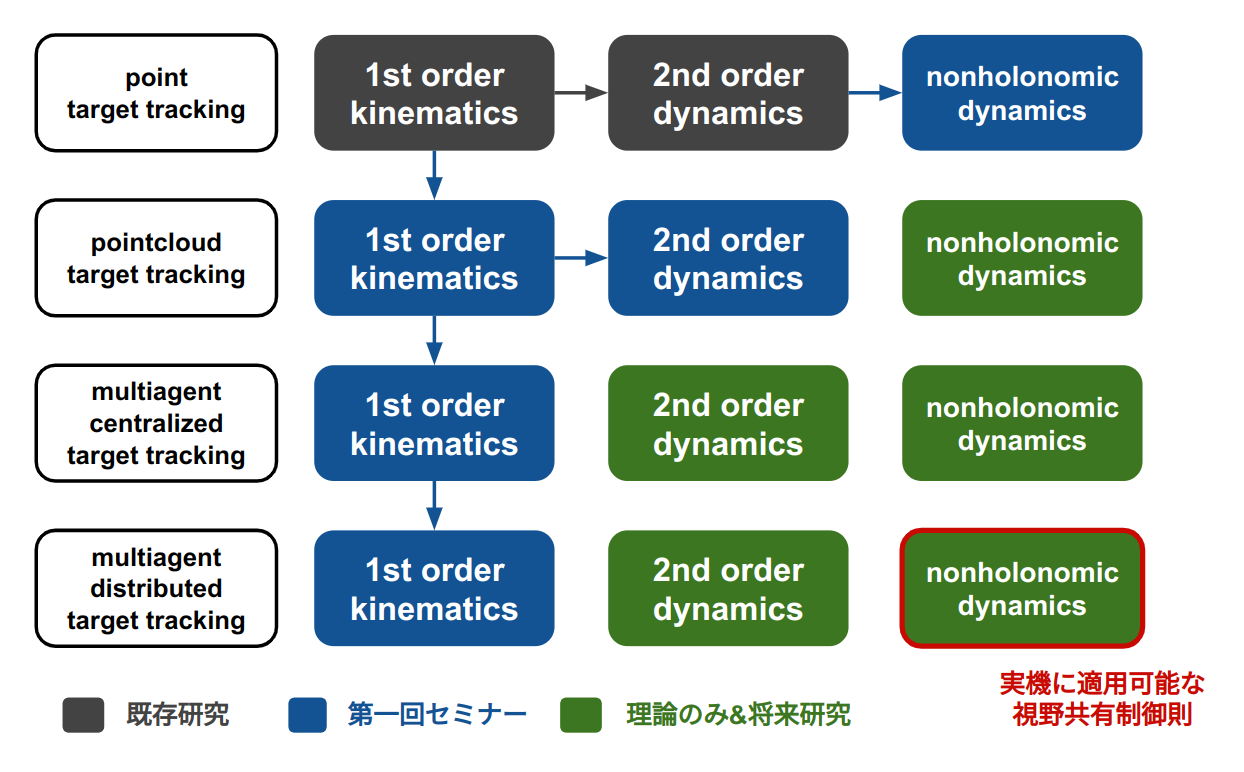
\includegraphics[width=0.8\linewidth]{fig/progress.png}
\caption{第一回セミナーの内容と本研究の貢献点}
\label{fig:progress}
\end{figure}
% \section{\textbf{準備:制御バリア関数}}
\section{準備:制御バリア関数}

本章では,本研究の基礎となる制御バリア関数(Control Barrier Function, CBF)の基本概念と高次制御バリア関数(High Order Control Barrier Function, HOCBF)について説明する.

\subsection{CBFの基本概念}

CBFは,システム状態がある安全集合内に留まることを保証するためのLyapunov関数に類似した概念である.以下では,CBFの基本的な定義と性質について述べる.

連続時間の制御アフィンシステムを考える:
\begin{equation}
\begin{aligned}
\dot{\mathbf{x}} = f(\mathbf{x}) + g(\mathbf{x})\mathbf{u}
\label{eq:control_affine}
\end{aligned}
\end{equation}
ここで,$\mathbf{x} \in \mathbb{R}^n$は状態,$\mathbf{u} \in \mathbb{R}^m$は制御入力,$f: \mathbb{R}^n \rightarrow \mathbb{R}^n$と$g: \mathbb{R}^n \rightarrow \mathbb{R}^{n \times m}$は局所Lipschitz連続な関数である.

安全集合$\mathcal{C}$を以下のように定義する:
\begin{equation}
\begin{aligned}
\mathcal{C} = \{\mathbf{x} \in \mathbb{R}^n : h(\mathbf{x}) \geq 0\}
\label{eq:safe_set}
\end{aligned}
\end{equation}
ここで,$h: \mathbb{R}^n \rightarrow \mathbb{R}$は連続微分可能な関数である.

\begin{dfn}[制御バリア関数]
関数$h: \mathbb{R}^n \rightarrow \mathbb{R}$が連続微分可能であり,その勾配$\nabla h(\mathbf{x})$が$\mathcal{C}$上でゼロにならないとする.このとき,$h$が制御バリア関数であるとは,ある拡張クラス$\mathcal{K}_{\infty}$関数$\alpha$が存在して,任意の$\mathbf{x} \in \mathcal{C}$に対して以下の条件を満たす制御入力$\mathbf{u} \in \mathbb{R}^m$が存在することである:
\begin{equation}
\begin{aligned}
L_f h(\mathbf{x}) + L_g h(\mathbf{x})\mathbf{u} + \alpha(h(\mathbf{x})) \geq 0
\label{eq:cbf_condition}
\end{aligned}
\end{equation}
ここで,$L_f h(\mathbf{x}) = \nabla h(\mathbf{x})^T f(\mathbf{x})$と$L_g h(\mathbf{x}) = \nabla h(\mathbf{x})^T g(\mathbf{x})$はそれぞれ$h$の$f$と$g$に関するLie微分である.
\end{dfn}

CBFの重要な性質は,\Eqref{eq:cbf_condition}を満たす任意の制御入力$\mathbf{u}$を用いると,安全集合$\mathcal{C}$が前方不変となることである.つまり,初期状態$\mathbf{x}(0) \in \mathcal{C}$に対して,任意の時刻$t \geq 0$において$\mathbf{x}(t) \in \mathcal{C}$が保証される.

実際の制御設計では,CBF制約を満たしつつ,制御目標を達成するための最適制御入力を求めることが多い.これは以下のような二次計画問題(Quadratic Programming, QP)として定式化できる:
\begin{equation}
\begin{aligned}
\mathbf{u}^* &= \underset{\mathbf{u} \in \mathbb{R}^m}{\text{argmin}} \:\: \|\mathbf{u} - \mathbf{u}_{\text{nom}}\|^2 \\
\text{s.t.} & \:\: L_f h(\mathbf{x}) + L_g h(\mathbf{x})\mathbf{u} + \alpha(h(\mathbf{x})) \geq 0
\label{eq:cbf_qp}
\end{aligned}
\end{equation}
ここで,$\mathbf{u}_{\text{nom}}$は安全制約を考慮しない場合の公称制御入力である.

\subsection{高次制御バリア関数}

従来のCBFは制約関数の相対次数が1であることを仮定していたが,多くの実システムでは安全制約が高次微分に依存するため,高次制御バリア関数(HOCBF)が必要となる.

関数$h(\mathbf{x})$の相対次数が$r > 1$の場合,以下のように補助関数の連鎖を定義する:
\begin{equation}
\begin{aligned}
\psi_0(\mathbf{x}) &= h(\mathbf{x}) \\
\psi_1(\mathbf{x}) &= \dot{\psi}_0(\mathbf{x}) + \alpha_1(\psi_0(\mathbf{x})) \\
\psi_2(\mathbf{x}) &= \dot{\psi}_1(\mathbf{x}) + \alpha_2(\psi_1(\mathbf{x})) \\
&\vdots \\
\psi_{r-1}(\mathbf{x}) &= \dot{\psi}_{r-2}(\mathbf{x}) + \alpha_{r-1}(\psi_{r-2}(\mathbf{x}))
\label{eq:hocbf_psi}
\end{aligned}
\end{equation}
ここで,$\alpha_i$($i = 1, 2, \ldots, r-1$)は拡張クラス$\mathcal{K}$関数である.

\begin{dfn}[高次制御バリア関数]
関数$h: \mathbb{R}^n \rightarrow \mathbb{R}$が$r$回連続微分可能であり,その相対次数が$r$であるとする.このとき,$h$が高次制御バリア関数であるとは,拡張クラス$\mathcal{K}$関数$\alpha_1, \alpha_2, \ldots, \alpha_r$が存在して,以下の条件を満たすことである:
\begin{equation}
\begin{aligned}
L_f^r h(\mathbf{x}) + L_g L_f^{r-1} h(\mathbf{x})\mathbf{u} + \alpha_r(\psi_{r-1}(\mathbf{x})) \geq 0
\label{eq:hocbf_condition}
\end{aligned}
\end{equation}
ここで,$L_f^r h(\mathbf{x})$は$h$の$f$に関する$r$次のLie微分,$L_g L_f^{r-1} h(\mathbf{x})$は$L_f^{r-1} h(\mathbf{x})$の$g$に関するLie微分である.
\end{dfn}

HOCBFを用いた制御設計では,\Eqref{eq:hocbf_condition}の制約を満たす制御入力を求めることで,安全集合$\mathcal{C}$の前方不変性を保証できる.これは以下のようなQP問題として定式化できる:
\begin{equation}
\begin{aligned}
\mathbf{u}^* = \arg\min_{\mathbf{u} \in \mathbb{R}^m} & \|\mathbf{u} - \mathbf{u}_{\text{nom}}\|^2 \\
\text{s.t.} & L_f^r h(\mathbf{x}) + L_g L_f^{r-1} h(\mathbf{x})\mathbf{u} + \alpha_r(\psi_{r-1}(\mathbf{x})) \geq 0
\label{eq:hocbf_qp}
\end{aligned}
\end{equation}

HOCBFは,非ホロノミック制約を持つシステムや,高次の安全制約を持つシステムに対して有効である.特に,本研究で扱うSE(3)上の剛体運動制御では,視野制約が状態の高次微分に依存するため,HOCBFが重要な役割を果たす.

\section{Problem Formulation}

本章では,本研究で扱うシステムモデルと問題設定について説明する.

\subsection{システムモデル(SE(3)上の剛体運動)}

本研究では,複数のエージェント(ドローン)がSE(3)上で運動する状況を考える.各エージェント$i \in \mathcal{A}$の位置と姿勢を$T_i = (p_i, R_i) \in \mathrm{SE}(3)$で表す.ここで,$p_i \in \mathbb{R}^3$はエージェント$i$の位置,$R_i \in \mathrm{SO}(3)$は姿勢を表す回転行列である.

SE(3)上の剛体運動は,以下の微分方程式で記述される.
\begin{equation}
\begin{aligned}
T &= \begin{bmatrix}
R & p \\
0 & 1
\end{bmatrix} \in \mathrm{SE}(3) \\
\xi^\wedge_B &= \begin{bmatrix}
[\omega]_\times & v_b \\
0 & 0
\end{bmatrix} \in \mathfrak{se}(3) \\
\dot{T} &= T \xi^\wedge_B
\label{eq:se3_dynamics}
\end{aligned}
\end{equation}
ここで,$\xi^\wedge_B$はボディ座標系における速度入力であり,$\omega \in \mathbb{R}^3$は角速度,$v_b \in \mathbb{R}^3$はボディ座標系における並進速度,$[\omega]_\times$は$\omega$に対応する歪対称行列である.

世界座標系における速度入力$\xi^\wedge_W$による剛体運動式は以下のように表される.
\begin{equation}
\begin{aligned}
\dot{T} &= \xi^\wedge_W T \\
\xi_W^\wedge &= (\mathrm{Ad}_T \xi_B)^\wedge \\
&= \left( \begin{bmatrix}
R & 0 \\
[p]_\times R & R
\end{bmatrix}
\begin{bmatrix}
\omega \\
v_b
\end{bmatrix} \right)^\wedge \\
&= \begin{bmatrix}
R\omega \\
[p]_\times R\omega + Rv_b
\end{bmatrix}^\wedge \\
&= \begin{bmatrix}
[R\omega]_\times & [p]_\times R\omega + Rv_b \\
0 & 0
\end{bmatrix}
\label{eq:se3_dynamics_world}
\end{aligned}
\end{equation}
ここで,$\mathrm{Ad}_T$はSE(3)の随伴表現である.

ボディ座標系における運動方程式を離散化すると,以下のようになる.
\begin{equation}
\begin{aligned}
T_{k+1} &\simeq T_k + \dot{T}_k \\
&\simeq T_k + h T_k \xi^\wedge_{B,k} \\
&= T_k + h \begin{bmatrix}
R_k & p_k \\
0 & 1
\end{bmatrix}
\begin{bmatrix}
[\omega_k]_\times & v_k \\
0 & 0
\end{bmatrix}
\label{eq:se3_discrete}
\end{aligned}
\end{equation}
ここで,$h$は離散時間ステップである.

成分分解すると,以下のように表される.
\begin{equation}
\begin{aligned}
R_{k+1} &\simeq R_k \exp(h[\omega_k]_{\times}) \\
&\simeq R_k(I + h[\omega_k]_{\times}) \\
p_{k+1} &= h R_k v_k + p_k
\label{eq:se3_discrete_components}
\end{aligned}
\end{equation}
ここで,$\exp(h[\omega_k]_{\times})$は$h[\omega_k]_{\times}$の行列指数関数であり,小さな$h$に対して$I + h[\omega_k]_{\times}$で近似できる.

\subsection{共有視野の定義と問題設定}

環境内には複数の特徴点$q_l \in \mathbb{R}^3, l \in \mathcal{L}$が存在する.エージェント$i$の観測している特徴点集合を$\mathcal{C}_i$とする.特徴点$q_l$がエージェント$i$の視野内にある条件は以下のように表される.
\begin{equation}
\begin{aligned}
q_l \in \mathcal{C}_i \iff \beta_l^{\top}(p_i)R_i e_c - \cos\Psi_\mathcal{F} > 0
\label{eq:fov_condition}
\end{aligned}
\end{equation}
ここで,$\beta_l(p_i) = \frac{q_l - p_i}{\|q_l - p_i\|}$は特徴点$q_l$からエージェント$i$への単位方向ベクトル,$e_c = [0 \; 0 \; 1]^\top$はカメラの光軸方向(ボディ座標系のz軸方向),$\Psi_\mathcal{F}$はカメラの視野角の半分である.

特徴点$q_l$が複数のエージェント$i, j \in \mathcal{A}$の共有視野内にある条件は以下のように表される.
\begin{equation}
\begin{aligned}
q_l \in \mathcal{C}_i \cap \mathcal{C}_j \iff (\beta_l^{\top}(p_i)R_i e_c - \cos\Psi_\mathcal{F})(\beta_l^{\top}(p_j)R_j e_c - \cos\Psi_\mathcal{F}) > 0
\label{eq:shared_fov_condition}
\end{aligned}
\end{equation}

本研究の目的は,各エージェントが目標位置$p_i^d$に向かって移動しながら,常に一定数以上の特徴点を共有視野内に保持するような制御入力$\xi_i = (\omega_i, v_i)$を設計することである.さらに,この制御則を分散型で実装することで,各エージェントが局所的な情報のみを用いて制御入力を決定できるようにする.

具体的には,以下の問題を解く.
\begin{equation}
\begin{aligned}
\min_{\xi_i, i \in \mathcal{A}} \sum_{i \in \mathcal{A}} \|p_i^d - p_i\|^2 + \|\xi_i\|^2 \\
\text{s.t.} \; |\mathcal{C}_i \cap \mathcal{C}_j| \geq m, \; \forall (i,j) \in \mathcal{E}
\label{eq:problem}
\end{aligned}
\end{equation}
ここで,$\mathcal{E}$はエージェント間の通信グラフの辺集合,$m$は共有視野内に保持すべき特徴点の最小数である.

この問題を解くために,次章では共有視野を保証するためのCBFを設計し,それに基づく制御則を提案する.

\section{CBFs for Shared Field of View}

本章では,共有視野を保証するための制御バリア関数(CBF)を設計する.まず単一の特徴点を追従する場合の安全制約を導出し,次に複数の特徴点を追従する場合,さらに複数のエージェントが共通の特徴点を追従する場合へと拡張する.最後に,分散型実装について述べる.

\subsection{単一特徴点追従の安全制約}

単一の特徴点を追従する安全制約については,Trimarchiら\cite{Trimarchi2025}の研究に大きく影響を受けている.

エージェント位置を$T_i=(p_i, R_i)\in \mathrm{SE}(3), i\in\mathcal{A}$,環境内の特徴点を$q_l\in \mathcal{L}$とする.エージェント$i$の観測している特徴点集合を$\mathcal{C}_i$とする.$q_l\in\mathcal{C}_i$である条件は,\Eqref{eq:fov_condition}で示したように以下のように表される.
\begin{equation}
\begin{aligned}
\beta_l^{\top}(p_i)R_ie_c-\cos\Psi_\mathcal{F}>0
\label{eq:fov_condition_single}
\end{aligned}
\end{equation}

この条件に基づいて,安全集合を以下のように定義する.
\begin{equation}
\begin{aligned}
B_{i} = \beta_l^{\top}(p_i)R_ie_c-\cos\Psi_\mathcal{F}
\label{eq:safe_set_single}
\end{aligned}
\end{equation}

安全集合$B_i$の時間微分は以下のように計算される.
\begin{equation}
\begin{aligned}
\dot{B}_{i} &= \langle \mathrm{grad}_R\:B_i,\omega_i\rangle + \langle \mathrm{grad}_p\:B_i,v_i\rangle \\
&= -\beta_l^\top(p_i) R_i [e_c]_\times\omega_i - \frac{e_c^\top R_i^\top P_{\beta_l}}{d_{i,l}}v_i
\label{eq:safe_set_derivative_single}
\end{aligned}
\end{equation}
ここで,$d_{i,l}={\|q_l-p_i\|}$は特徴点$q_l$とエージェント$i$の距離,$P_{\beta_l} = I-\beta_l\beta_l^\top$は$\beta_l$に直交する平面への投影行列である.また,$\mathrm{grad}_R\:B_i$と$\mathrm{grad}_p\:B_i$はそれぞれ$B_i$の$R_i$と$p_i$に関する勾配である.

CBFの条件より,安全制約は以下のように表される.
\begin{equation}
\begin{aligned}
-\beta_l^\top(p_i) R_i [e_c]_\times\omega_i - \frac{e_c^\top R_i^\top P_{\beta_l}}{d_{i,l}}v_i \leq \gamma (\beta_l^{\top}(p_i)R_ie_c-\cos\Psi_\mathcal{F})
\label{eq:cbf_constraint_single}
\end{aligned}
\end{equation}
ここで,$\gamma > 0$はCBFのゲインパラメータである.

CBF制約を満たしつつ,目標位置$p_i^d$に追従するためのQPは以下のように定式化される.
\begin{equation}
\begin{aligned}
\min_{\xi_i} \: (p^d_{i}-p_{i,{k}}-hR_{i,k}v_{i,k})^\top Q_1 & (p^d_{i}-p_{i,{k}}-hR_{i,k}v_{i,k})
+ 
\begin{bmatrix}
\omega_{i,k}\\v_{i,k}
\end{bmatrix}^\top Q_2
\begin{bmatrix}
\omega_{i,k}\\v_{i,k}
\end{bmatrix} \\
\mathrm{s.t.} \quad
\beta_l^\top(p_i) R_i [e_c]_\times\omega_i &+ \frac{e_c^\top R_i^\top P_{\beta_l}}{d_{i,l}}v_i \leq \gamma (\beta_l^{\top}(p_i)R_ie_c-\cos\Psi_\mathcal{F})
\label{eq:qp_single}
\end{aligned}
\end{equation}
ここで,$Q_1$と$Q_2$は正定値重み行列である.

この最適化問題を一般的な形式に変換すると,以下のようになる.
\begin{equation}
\begin{aligned}
&\min_{\xi_i}\:J_i \\
J_i &= \frac{1}{2}\xi_{i,k}^\top H_i \xi_{i,k} + f_i^\top \xi_{i,k} \\
\xi_{i,k} &= \begin{bmatrix}
\omega_{i,k}\\v_{i,k}
\end{bmatrix}, \quad
H_i = 2\begin{bmatrix}
Q_{2,\omega} & Q_{2,\omega v} \\ 
Q^\top_{2,\omega v} & Q_{2,v}+h^2R_{i,k}^\top Q_1R_{i,k}
\end{bmatrix}, \\
f_i &= \begin{bmatrix}
0 \\ -2hR_i^\top Q_1 e_i
\end{bmatrix}, \quad e_i = p^d_{i}-p_{i,k} \\
\mathrm{s.t.} &\quad
\begin{bmatrix}
\beta_l^\top(p_i) R_i [e_c]_\times \\
\frac{e_c^\top R_i^\top P_{\beta_l}}{d_{i,l}}
\end{bmatrix}^\top \xi_{i,k} \leq
\gamma (\beta_l^{\top}(p_i)R_ie_c-\cos\Psi_\mathcal{F})
\label{eq:qp_single_general}
\end{aligned}
\end{equation}

\subsection{複数特徴点追従の安全制約}

複数の特徴点を追従することを考える場合,単純に各特徴点に対する安全集合の積集合を考えることもできるが,それでは安全集合が微分不可能になる可能性がある.そこで,確率的なアプローチを導入する.

特徴点$q_l \in \mathcal{L}$によってエージェント$i$における推定が成り立っている確率を以下のように定義する.
\begin{equation}
\begin{aligned}
\phi_{i}^l = P(p_i,R_i,q_l)
\label{eq:probability_single}
\end{aligned}
\end{equation}

この確率を用いて,新しい安全集合を以下のように定義する.
\begin{equation}
\begin{aligned}
B_{i} = 1-q-\prod_{l\in\mathcal{L}}(1-\phi_{i}^l)
\label{eq:safe_set_multi}
\end{aligned}
\end{equation}
ここで,$q \in (0,1)$はパラメータであり,環境内の特徴点$q_l \in \mathcal{L}$によってエージェント$i$における推定が達成される確率を$q$以上に制限することを意味する.

確率$\phi_{i}^l$は以下のように定義する.
\begin{equation}
\begin{aligned}
P(p_i,R_i,q_l) &= \left\{ \begin{array}{ll}
P_i^l & \mathrm{if} \quad q_l\in\mathcal{C}_i \\
0 & \mathrm{if} \quad q_l\in \mathcal{L}\setminus\mathcal{C}_i
\end{array} \right. \\
\mathrm{where} \quad P_i^l &= \frac{\beta_l^\top(p_i) R_i e_c -\cos\Psi_\mathcal{F}}{1-\cos\Psi_\mathcal{F}}
\label{eq:probability_definition}
\end{aligned}
\end{equation}

安全制約は以下のように表される.
\begin{equation}
\begin{aligned}
B_{i} > 0 \quad \forall i \in \mathcal{A}
\label{eq:safe_constraint_multi}
\end{aligned}
\end{equation}

安全集合$B_i$の時間微分は以下のように計算される.
\begin{equation}
\begin{aligned}
B_{i} &= 1-q-\eta_{i} \\
\eta_{i} &= \prod_{l\in\mathcal{L}}(1-\phi_{i}^l) \\
\dot{B}_{i} &= -\dot{\eta}_{i} \\
&= -\frac{d}{dt}\prod_{l\in\mathcal{L}}(1-\phi_{i}^l) \\
&= \sum_{l\in \mathcal{L}}(\prod_{k\neq l}(1-\phi_{i}^k))\dot{\phi}^l_{i} \\
\dot{\phi}^l_{i} &= \left\{ \begin{array}{ll}
\dot{P}_i^l & \mathrm{if} \quad q_l\in\mathcal{C}_i \\
0 & \mathrm{if} \quad q_l\in \mathcal{L}\setminus\mathcal{C}_i
\end{array} \right.
\label{eq:safe_set_derivative_multi}
\end{aligned}
\end{equation}

$P_i^l$の微分は以下のように計算できる.
\begin{equation}
\begin{aligned}
P_i^l &= \frac{\beta_l^\top(p_i) R_i e_c -\cos\Psi_\mathcal{F}}{1-\cos\Psi_\mathcal{F}} \\
\dot{P}_i^l &= \langle \mathrm{grad}\:P_i^l, \xi_W\rangle \\
&= \left\langle 
\begin{bmatrix}\mathrm{grad}_R\:P_i^l\\\mathrm{grad}_p\:P_i^l
\end{bmatrix},
\begin{bmatrix}\omega_i\\v_i
\end{bmatrix}
\right\rangle \\
\mathrm{grad}_p\:P_i^l &= \frac{1}{1-\cos \Psi_\mathcal{F}}\left(-\frac{e_c^\top R_i^\top P_{\beta_l}}{d_{i,l}}\right) \\
\mathrm{grad}_R\:P_i^l &= \frac{1}{1-\cos \Psi_\mathcal{F}}(-\beta_l^\top(p_i) R_i [e_c]_\times)
\label{eq:probability_derivative}
\end{aligned}
\end{equation}

これらから,複数の特徴点を追従するためのCBF制約は以下のようになる.
\begin{equation}
\begin{aligned}
\sum_{l\in \mathcal{L}\cap\mathcal{C}_i}(\prod_{k\neq l}(1-\phi_{i}^k)) \langle \mathrm{grad}_R\:P_i^l,\omega_i\rangle &+ \sum_{l\in \mathcal{L}\cap\mathcal{C}_i}(\prod_{k\neq l}(1-\phi_{i}^k)) \langle \mathrm{grad}_p\:P_i^l,v_i\rangle \\
&\geq -\gamma_0 (1-q-\prod_{l\in\mathcal{L}}(1-\phi_{i}^l))
\label{eq:cbf_constraint_multi}
\end{aligned}
\end{equation}
ここで,$\gamma_0 > 0$はCBFのゲインパラメータである.

CBF制約を満たしつつ,目標位置$p_i^d$に追従するためのQPは以下のように定式化される.
\begin{equation}
\begin{aligned}
\min_{\xi_i} \: (p^d_{i}-p_{i,{k+1}})^\top Q_1 & (p^d_{i}-p_{i,{k+1}})
+ \xi_{i,k}^\top Q_2 \xi_{i,k} \\
\mathrm{s.t.} \quad
\sum_{l\in \mathcal{L}\cap\mathcal{C}_i}(\prod_{k\neq l}(1-\phi_{i}^k)) \frac{\beta_l^\top(p_i) R_i [e_c]_\times}{1-\cos \Psi_\mathcal{F}}\omega_i &+ \sum_{l\in \mathcal{L}\cap\mathcal{C}_i}(\prod_{k\neq l}(1-\phi_{i}^k)) \frac{e_c^\top R_i^\top P_{\beta_l}}{(1-\cos \Psi_\mathcal{F})d_{i,l}}v_i \\
&\leq \gamma_0 (1-q-\prod_{l\in\mathcal{L}}(1-\phi_{i}^k))
\label{eq:qp_multi}
\end{aligned}
\end{equation}

一般的なQPの形式に変換すると,以下のようになる.
\begin{equation}
\begin{aligned}
&\min_{\xi_i}\:J_i \\
J_i &= \frac{1}{2}\xi_{i,k}^\top H_i \xi_{i,k} + f_i^\top \xi_{i,k} \\
\xi_{i,k} &= \begin{bmatrix}
\omega_{i,k}\\v_{i,k}
\end{bmatrix}, \quad
H_i = 2\begin{bmatrix}
Q_{2,\omega} & Q_{2,\omega v} \\ 
Q^\top_{2,\omega v} & Q_{2,v}+h^2R_{i,k}^\top Q_1R_{i,k}
\end{bmatrix}, \\
f_i &= \begin{bmatrix}
0 \\ -2hR_i^\top Q_1 e_i
\end{bmatrix}, \quad e_i = p^d_{i}-p_{i,k} \\
\mathrm{s.t.} &\quad
\begin{bmatrix}
\sum_{l\in \mathcal{L}\cap\mathcal{C}_i}(\prod_{k\neq l}(1-\phi_{i}^k)) \frac{\beta_l^\top(p_i) R_i [e_c]_\times}{1-\cos \Psi_\mathcal{F}} \\
\sum_{l\in \mathcal{L}\cap\mathcal{C}_i}(\prod_{k\neq l}(1-\phi_{i}^k))\frac{e_c^\top R_i^\top P_{\beta_l}}{(1-\cos \Psi_\mathcal{F})d_{i,l}}
\end{bmatrix}^\top \xi_{i,k} \leq
\gamma_0(1-q-\prod_{l\in \mathcal{L}}(1-\phi_{i}^k))
\label{eq:qp_multi_general}
\end{aligned}
\end{equation}

\subsection{複数エージェントの共通特徴点追従}

次に,複数のエージェントが共通の特徴点を追従する場合を考える.エージェント$i$と$j$が特徴点$q_l$を共有視野内に持つ条件は,\Eqref{eq:shared_fov_condition}で示したように以下のように表される.
\begin{equation}
\begin{aligned}
(\beta_l^{\top}(p_i)R_ie_c-\cos\Psi_\mathcal{F})(\beta_l^{\top}(p_j)R_je_c-\cos\Psi_\mathcal{F}) > 0
\label{eq:shared_fov_condition_repeat}
\end{aligned}
\end{equation}

特徴点$q_l \in \mathcal{L}$によってエッジ$(i,j) \in \mathcal{E}$における推定が成り立っている確率を以下のように定義する.
\begin{equation}
\begin{aligned}
\phi_{ij}^l = P(p_i,R_i,p_j,R_j,q_l)
\label{eq:probability_edge}
\end{aligned}
\end{equation}

この確率を用いて,新しい安全集合を以下のように定義する.
\begin{equation}
\begin{aligned}
B_{ij} = 1-q-\prod_{l\in\mathcal{L}}(1-\phi_{ij}^l)
\label{eq:safe_set_edge}
\end{aligned}
\end{equation}
ここで,$q \in (0,1)$はパラメータであり,環境内の特徴点$q_l \in \mathcal{L}$によってエッジ$(i,j) \in \mathcal{E}$における推定が達成される確率を$q$以上に制限することを意味する.

確率$\phi_{ij}^l$は以下のように定義する.
\begin{equation}
\begin{aligned}
P(p_i,R_i,p_j,R_j,q_l) &= \left\{ \begin{array}{ll}
P_i^l P_j^l & \mathrm{if} \quad q_l\in\mathcal{C}_i \cap \mathcal{C}_j \\
0 & \mathrm{if} \quad q_l\in \mathcal{L}\setminus(\mathcal{C}_i \cap \mathcal{C}_j)
\end{array} \right. \\
\mathrm{where} \quad P_i^l &= \frac{\beta_l^\top(p_i) R_i e_c -\cos\Psi_\mathcal{F}}{1-\cos\Psi_\mathcal{F}}
\label{eq:probability_edge_definition}
\end{aligned}
\end{equation}

安全制約は以下のように表される.
\begin{equation}
\begin{aligned}
B_{ij} > 0 \quad \forall (i,j) \in \mathcal{E}
\label{eq:safe_constraint_edge}
\end{aligned}
\end{equation}

安全集合$B_{ij}$の時間微分は以下のように計算される.
\begin{equation}
\begin{aligned}
B_{ij} &= 1-q-\eta_{ij} \\
\eta_{ij} &= \prod_{l\in\mathcal{L}}(1-\phi_{ij}^l) \\
\dot{B}_{ij} &= -\dot{\eta}_{ij} \\
&= -\frac{d}{dt}\prod_{l\in\mathcal{L}}(1-\phi_{ij}^l) \\
&= \sum_{l\in \mathcal{L}}(\prod_{k\neq l}(1-\phi_{ij}^k))\dot{\phi}^l_{ij} \\
\dot{\phi}^l_{ij} &= \left\{ \begin{array}{ll}
\dot{P}_i^l P_j^l + P_i^l \dot{P}_j^l & \mathrm{if} \quad q_l\in\mathcal{C}_i \cap \mathcal{C}_j \\
0 & \mathrm{if} \quad q_l\in \mathcal{L}\setminus(\mathcal{C}_i \cap \mathcal{C}_j)
\end{array} \right.
\label{eq:safe_set_derivative_edge}
\end{aligned}
\end{equation}

エージェントごとの制御入力について分解すると,以下のようになる.
\begin{equation}
\begin{aligned}
\dot{B}_{ij} &= -\dot{\eta}_{ij} \\
&= -\frac{d}{dt}\prod_{l\in\mathcal{L}}(1-\phi_{ij}^l) \\
&= \sum_{l\in \mathcal{L}}(\prod_{k\neq l}(1-\phi_{ij}^k))\dot{\phi}^l_{ij} \\
&= \sum_{l\in \mathcal{L}\cap\mathcal{C}_i \cap \mathcal{C}_j}(\prod_{k\neq l}(1-\phi_{ij}^k))P_j^l\dot{P}_i^l + \sum_{l\in \mathcal{L}\cap\mathcal{C}_i \cap \mathcal{C}_j}(\prod_{k\neq l}(1-\phi_{ij}^k))P_i^l\dot{P}_j^l
\label{eq:safe_set_derivative_edge_decomposed}
\end{aligned}
\end{equation}

これらから,複数のエージェントが共通の特徴点を追従するためのCBF制約は以下のようになる.
\begin{equation}
\begin{aligned}
&\sum_{l\in \mathcal{L}\cap\mathcal{C}_i \cap \mathcal{C}_j}(\prod_{k\neq l}(1-\phi_{ij}^k))P_j^l \langle \mathrm{grad}_R\:P_i^l,\omega_i\rangle + \sum_{l\in \mathcal{L}\cap\mathcal{C}_i \cap \mathcal{C}_j}(\prod_{k\neq l}(1-\phi_{ij}^k))P_i^l \langle \mathrm{grad}_R\:P_j^l,\omega_j \rangle \\
&+ \sum_{l\in \mathcal{L}\cap\mathcal{C}_i \cap \mathcal{C}_j}(\prod_{k\neq l}(1-\phi_{ij}^k))P_j^l \langle \mathrm{grad}_p\:P_i^l,v_i\rangle + \sum_{l\in \mathcal{L}\cap\mathcal{C}_i \cap \mathcal{C}_j}(\prod_{k\neq l}(1-\phi_{ij}^k))P_i^l \langle \mathrm{grad}_p\:P_j^l, v_j\rangle \\
&\geq -\gamma_0 (1-q-\prod_{l\in\mathcal{L}}(1-\phi_{ij}^l))
\label{eq:cbf_constraint_edge}
\end{aligned}
\end{equation}
ここで,$\gamma_0 > 0$はCBFのゲインパラメータである.

CBF制約を満たしつつ,目標位置$p_i^d$と$p_j^d$に追従するためのQPは以下のように定式化される.
\begin{equation}
\begin{aligned}
\min_{\xi_i, \xi_j} \: \sum_{i,j}(p^d_{i}-p_{i,{k+1}}-hR_{i,k}v_{i,k})^\top Q_1 & (p^d_{i}-p_{i,{k+1}}-hR_{i,k}v_{i,k})
+ 
\begin{bmatrix}
\omega_{i,k}\\v_{i,k}
\end{bmatrix}^\top Q_2
\begin{bmatrix}
\omega_{i,k}\\v_{i,k}
\end{bmatrix} \\
\mathrm{s.t.} \quad
&\sum_{l\in \mathcal{L}\cap\mathcal{C}_i \cap \mathcal{C}_j}(\prod_{k\neq l}(1-\phi_{ij}^k)) \frac{P_j^l\beta_l^\top(p_i) R_i [e_c]_\times}{1-\cos \Psi_\mathcal{F}}\omega_i \\
&+ \sum_{l\in \mathcal{L}\cap\mathcal{C}_i \cap \mathcal{C}_j}(\prod_{k\neq l}(1-\phi_{ij}^k)) 
\frac{P_i^l\beta_l^\top(p_j) R_j [e_c]_\times}{1-\cos \Psi_\mathcal{F}}\omega_j \\
&+ \sum_{l\in \mathcal{L}\cap\mathcal{C}_i \cap \mathcal{C}_j}(\prod_{k\neq l}(1-\phi_{ij}^k))\frac{P_j^le_c^\top R_i^\top P_{\beta_l}}{(1-\cos \Psi_\mathcal{F})d_{i,l}}v_i \\
&+ \sum_{l\in \mathcal{L}\cap\mathcal{C}_i \cap \mathcal{C}_j}(\prod_{k\neq l}(1-\phi_{ij}^k))\frac{P_i^le_c^\top R_j^\top P_{\beta_l}}{(1-\cos \Psi_\mathcal{F})d_{j,l}}v_j \\
&\leq \gamma_0 (1-q-\prod_{l\in\mathcal{L}}(1-\phi_{ij}^l))
\label{eq:qp_edge}
\end{aligned}
\end{equation}

一般的なQPの形式に変換すると,以下のようになる.
\begin{equation}
\begin{aligned}
&\min_{\xi_i, \xi_j} \: \sum_{i,j}J_i \\
J_i &= \frac{1}{2}\xi_{i,k}^\top H_i\xi_{i,k} + f_i^\top\xi_{i,k} \\
\xi_{i,k} &= \begin{bmatrix}
\omega_{i,k}\\v_{i,k}
\end{bmatrix}, \quad
H_i = 2\begin{bmatrix}
Q_{2,\omega} & Q_{2,\omega v} \\ 
Q^\top_{2,\omega v} & Q_{2,v}+h^2R_{i,k}^\top Q_1R_{i,k}
\end{bmatrix}, \\
f_i &= \begin{bmatrix}
0 \\ -2hR_i^\top Q_1 e_i
\end{bmatrix}, \quad e_i = p^d_{i}-p_{i,k} \\
\mathrm{s.t.} &\quad \begin{bmatrix}
\alpha_\omega & \alpha_v & \beta_\omega & \beta_v
\end{bmatrix}
\begin{bmatrix}
\omega_{i,k} \\ v_{i,k} \\ \omega_{j,k} \\ v_{j,k}
\end{bmatrix} \leq
\gamma_0\gamma
\label{eq:qp_edge_general}
\end{aligned}
\end{equation}
ここで,係数は以下のように定義される.
\begin{equation}
\begin{aligned}
\alpha_\omega &= \sum_{l\in \mathcal{L}\cap\mathcal{C}_i \cap \mathcal{C}_j}(\prod_{k\neq l}(1-\phi_{ij}^k)) \frac{P_j^l\beta_l^\top(p_i) R_i [e_c]_\times}{1-\cos \Psi_\mathcal{F}} \in \mathbb{R}^3 \\
\beta_\omega &= \sum_{l\in \mathcal{L}\cap\mathcal{C}_i \cap \mathcal{C}_j}(\prod_{k\neq l}(1-\phi_{ij}^k)) 
\frac{P_i^l\beta_l^\top(p_j) R_j [e_c]_\times}{1-\cos \Psi_\mathcal{F}} \in \mathbb{R}^3 \\
\alpha_v &= \sum_{l\in \mathcal{L}\cap\mathcal{C}_i \cap \mathcal{C}_j}(\prod_{k\neq l}(1-\phi_{ij}^k))\frac{P_j^le_c^\top R_i^\top P_{\beta_l}}{(1-\cos \Psi_\mathcal{F})d_{i,l}} \in \mathbb{R}^3 \\
\beta_v &= \sum_{l\in \mathcal{L}\cap\mathcal{C}_i \cap \mathcal{C}_j}(\prod_{k\neq l}(1-\phi_{ij}^k))\frac{P_i^le_c^\top R_j^\top P_{\beta_l}}{(1-\cos \Psi_\mathcal{F})d_{j,l}} \in \mathbb{R}^3 \\
\gamma &= 1-q-\prod_{l\in \mathcal{L}\cap\mathcal{C}_i \cap \mathcal{C}_j}(1-\phi_{ij}^l) \in \mathbb{R}
\label{eq:qp_edge_coefficients}
\end{aligned}
\end{equation}

\subsection{分散型実装}

不等式制約付き最適化問題を分散化する方法はいくつかあるが,本研究では主双対乗数法(Primal-Dual Method of Multipliers, PDMM)を用いる.PDMMは,不等式制約を処理する場合にADMMのようにスラック変数修正が必要なく,より効率的に解くことができる\cite{Zhang2024}.

IEQ-PDMM(inequality constraint primal-dual method of multipliers)を用いて上の式を分散化すると以下のようになる.
\begin{equation}
\begin{aligned}
\xi_i &= \underset{\xi_i}{\mathrm{argmin}} \:J_i(\xi_i)+z_{i|j}^\top A_{ij}\xi_i+\frac{c}{2}\|A_{ij}\xi_i-\frac{1}{2}\gamma_0\gamma\|^2 \\
y_{i|j} &= z_{i|j}+2c(A_{ij}\xi_{i}-\frac{1}{2}\gamma_0\gamma) \\
&\mathbf{node}_j\leftarrow \mathbf{node}_i(y_{i|j}) \\
&\mathbf{if}\:y_{i|j}+y_{j|i}>0 \\
&\qquad z_{i|j}=y_{j|i} \\
&\mathbf{else}\: \\
&\qquad z_{i|j}=-y_{i|j}
\label{eq:pdmm}
\end{aligned}
\end{equation}
ここで,$A_{ij} = \begin{bmatrix} \alpha_\omega \\ \alpha_v \end{bmatrix}$,$A_{ji} = \begin{bmatrix} \beta_\omega \\ \beta_v \end{bmatrix}$である.

QPの形式に表すと,以下のようになる.
\begin{equation}
\begin{aligned}
&\min_{\xi_i}\:\hat{J}_i = \frac{1}{2}\xi_{i,k}^\top \hat{H}_i\xi_{i,k} + \hat{f}_i^\top \xi_{i,k} \\
\xi_{i,k} &= \begin{bmatrix}
\omega_{i,k}\\v_{i,k}
\end{bmatrix}, \quad
\hat{H}_i = \begin{bmatrix}
2Q_{2,\omega}+c\alpha_\omega^\top \alpha_\omega & 2Q_{2,\omega v}+c\alpha_\omega^\top \alpha_v \\
2Q^\top_{2,\omega v}+c\alpha_v^\top \alpha_\omega & 2Q_{2,v}+2h^2R_{i,k}^\top Q_1R_{i,k}+c\alpha_v^\top \alpha_v
\end{bmatrix}, \\
\hat{f}_i &= \begin{bmatrix}
z_{i|j}\alpha_\omega^\top -\frac{c}{2}\gamma_0\gamma\alpha_\omega^\top \\
-2hR_i^\top Q_1 e_i+z_{i|j}\alpha_v^\top -\frac{c}{2}\gamma_0\gamma\alpha_v^\top
\end{bmatrix}, \quad e_i = p^d_{i}-p_{i,k}
\label{eq:pdmm_qp}
\end{aligned}
\end{equation}

この計算手法では制約式がすべてソフト制約化するため,最適化中に元の制約式を満たすことを保証できない.そこで,Tanら\cite{Tan2022}が提案したCBF-induced QPを用いることも考えられる.これは,ADMMベースのCBF分散化手法であり,最適化中に元の制約式を満たすことを保証する.

本章では,共有視野を保証するためのCBFを設計し,それに基づく制御則を提案した.次章では,二次系システムのための高次CBFを導入し,より実際的なドローンダイナミクスに対応する手法を提案する.

\section{二次系システムのための高次CBF}

本章では,共有視野の分散CBFを実機に適用するため,ドローンのダイナミクスを考慮した高次制御バリア関数(HOCBF)付きQPの定式化について述べる.まず,SE(3)における離散ダイナミクスを導出し,次にホロノミック系とQP定式化,非ホロノミック系への拡張,さらに複数エージェント・複数特徴点の場合へと拡張する.

\subsection{SE(3)における離散ダイナミクス}

SE(3)における離散ダイナミクスは以下のように表される:
\begin{equation}
\begin{aligned}
R_{k+1} &= R_k F_k \\
p_{k+1} &= p_k + h R_k v_k \\
M v_{k+1} &= F_k^\top M v_k + h \mathcal{U}_{k+1} + h f_k \\
J \Omega_{k+1} &= F_k^\top J \Omega_k + h M v_{k+1} \times v_{k+1} + h \mathcal{M}_{k+1} + h \tau_k
\label{eq:se3_discrete_dynamics}
\end{aligned}
\end{equation}
ここで,$R_k \in \mathrm{SO}(3)$は回転行列,$p_k \in \mathbb{R}^3$は位置ベクトル,$v_k \in \mathbb{R}^3$は並進速度ベクトル,$\Omega_k \in \mathbb{R}^3$は角速度ベクトル,$F_k \in \mathrm{SO}(3)$は回転の更新行列,$M \in \mathbb{R}^{3 \times 3}$は質量行列,$J \in \mathbb{R}^{3 \times 3}$は慣性モーメント行列,$\mathcal{U}(p, R) = -R^\top \frac{\partial U}{\partial p}(p, R)$と$\mathcal{M}(p, R)^\times = \frac{\partial U}{\partial R}^\top R - R^\top \frac{\partial U}{\partial R}$はポテンシャルエネルギー$U$から導出される力とトルク,$f_k \in \mathbb{R}^3$は外力,$\tau_k \in \mathbb{R}^3$は外部トルク,$h$はサンプリング時間である.

重力ポテンシャルを$U = mgp_z$とすると,$\mathcal{U} = mgR^\top e_z$,$\mathcal{M} = 0$となる.また,一般的な近似として,$F_k \simeq \exp(h\Omega_k^\times) \simeq I + h\Omega_k^\times$を用いる.

並進運動について,\Eqref{eq:se3_discrete_dynamics}の第3式を展開すると:
\begin{equation}
\begin{aligned}
M v_{k+1} &= F_k^\top M v_k + h \mathcal{U}_{k+1} + h f_k \\
&= M v_k + h (M v_k \times \Omega_k - M g R^\top e_z + f_k)
\label{eq:translation_dynamics}
\end{aligned}
\end{equation}

回転運動について,後述する非ホロノミック系に対応するため,以下のような近似を行う:
\begin{equation}
\begin{aligned}
R_{k+1} &= R_k F_k \simeq R_k F_{k+1} \\
p_{k+1} &= p_k + h R_k v_k \simeq p_k + h R_{k+1} v_{k+1}
\label{eq:approximation}
\end{aligned}
\end{equation}

この近似の下で,姿勢更新は以下のようになる:
\begin{equation}
\begin{aligned}
J \Omega_{k+1} &= F_k^\top J \Omega_k + \underbrace{h M v_{k+1} \times v_{k+1}}_{\simeq 0} + \underbrace{h \mathcal{M}_{k+1}}_{= 0} + h \tau_k \\
&= J \Omega_k + \underbrace{h J \Omega_k \times \Omega_k}_{\simeq 0} + h \tau_k \\
R_{k+1} &= R_k + h R_k \Omega_{k+1}^\times \\
&= R_k + h R_k [\Omega_k + h J^{-1} \tau_k]_\times \\
&= R_k + h R_k \Omega_k^\times + h^2 R_k [J^{-1} \tau_k]_\times
\label{eq:rotation_dynamics}
\end{aligned}
\end{equation}

位置更新は以下のようになる:
\begin{equation}
\begin{aligned}
p_{k+1} &= p_k + h R_{k+1} v_{k+1} \\
&= p_k + h (R_k + h R_k \Omega_{k+1}^\times) (v_k + h (v_k \times \Omega_k - g R_k^\top e_z + M^{-1} f_k)) \\
&= p_k + h R_k v_k + h^2 (-g e_z + R_k M^{-1} f_k) + h^3 [J^{-1} \tau_k]_\times v_k + \mathcal{O}(h^4)
\label{eq:position_dynamics}
\end{aligned}
\end{equation}

これにより,逐次ステップでトルク$\tau_k$と力$f_k$によって状態$(p_{k+1}, R_{k+1}) \in \mathrm{SE}(3)$を操作可能になる.

\subsection{ホロノミック系とQP定式化}

まず,$f = (f_x, f_y, f_z) \in \mathbb{R}^3$(ホロノミック系)におけるHOCBF-QPを考える.

目標位置$p^d_k$と現在位置$p_{k+1}$の誤差を以下のように定義する:
\begin{equation}
\begin{aligned}
p^d_k - p_{k+1} &= \underbrace{p^d_k - p_k - h R_k v_k}_{e_k} - h^2 (-g e_z + R_k M^{-1} f_k) - h^3 [J^{-1} \tau_k]_\times v_k \\
&= \underbrace{e_k + h^2 g e_z}_{\tilde{e}_k} - h^2 M^{-1} R_k f_k + h^3 v_k^\times J^{-1} \tau_k \\
&= \tilde{e}_k + A_f f_k + A_\tau \tau_k \\
&= \tilde{e}_k + \begin{bmatrix} A_f & A_\tau \end{bmatrix} \begin{bmatrix} f_k \\ \tau_k \end{bmatrix} \\
&= \tilde{e}_k + A u_k
\label{eq:error}
\end{aligned}
\end{equation}
ここで,$A_f = -h^2 M^{-1} R_k$,$A_\tau = h^3 v_k^\times J^{-1}$,$u_k = [f_k^\top, \tau_k^\top]^\top$である.

最小化したい目的関数は以下のようになる:
\begin{equation}
\begin{aligned}
J &= \frac{1}{2} \|\tilde{e}_k + A u_k\|^2 + \frac{1}{2} \begin{bmatrix} A_g + M^{-1} f_k \\ J^{-1} \tau_k \end{bmatrix}^\top B \begin{bmatrix} A_g + M^{-1} f_k \\ J^{-1} \tau_k \end{bmatrix} \\
&\propto \frac{1}{2} u_k^\top A^\top A u_k + (A^\top \tilde{e}_k)^\top u_k \\
&\quad + \frac{1}{2} u_k^\top \underbrace{\begin{bmatrix} M^{-2} B_1 & 0 \\ 0 & (J^{-1})^\top B_2 J^{-1} \end{bmatrix}}_{B'_1 \in \mathbb{R}^{6 \times 6}} u_k + \underbrace{\begin{bmatrix} M^{-1} B_1 A_g^\top e_z \\ 0 \end{bmatrix}^\top}_{B'_2 \in \mathbb{R}^6} u_k \\
&\propto \frac{1}{2} u_k^\top (A^\top A + B'_1) u_k + (A^\top \tilde{e}_k + B'_2)^\top u_k
\label{eq:objective}
\end{aligned}
\end{equation}
ここで,$A_g = v_k^\times \Omega_k - g R_k^\top e_z$である.

よって,解くべきQP問題は以下のようになる:
\begin{equation}
\begin{aligned}
\min_{u_k} \quad & \frac{1}{2} u_k^\top (A^\top A + B'_1) u_k + (A^\top \tilde{e}_k + B'_2)^\top u_k \\
\mathrm{s.t.} \quad & C u_k \leq b
\label{eq:holonomic_qp}
\end{aligned}
\end{equation}
ここで,
\begin{equation}
\begin{aligned}
u_k &= \begin{bmatrix} f_k \\ \tau_k \end{bmatrix} \in \mathbb{R}^6 \\
A &= \begin{bmatrix} -h^2 M^{-1} R_k & h^3 v_k^\times J^{-1} \end{bmatrix} \in \mathbb{R}^{3 \times 6} \\
B'_1 &= \begin{bmatrix} M^{-2} B_1 & 0 \\ 0 & (J^{-1})^\top B_2 J^{-1} \end{bmatrix} \in \mathbb{R}^{6 \times 6} \\
B'_2 &= \begin{bmatrix} M^{-1} B_1 A_g^\top e_z \\ 0 \end{bmatrix} \in \mathbb{R}^6 \\
\tilde{e}_k &= p^d_k - p_k - h R_k v_k + h^2 g e_z
\label{eq:holonomic_qp_params}
\end{aligned}
\end{equation}
である.$C$と$b$は安全制約から導出される.

\subsection{単一の特徴点を追従するHOCBF制約}

単一の特徴点$q_l$を追従する安全制約について考える.安全集合を以下のように定義する:
\begin{equation}
\begin{aligned}
h = \beta_l^\top(p_i) R_i e_c - \cos\Psi_\mathcal{F}
\label{eq:single_hocbf_safe_set}
\end{aligned}
\end{equation}

安全集合の2階微分は以下のように計算できる:
\begin{equation}
\begin{aligned}
\ddot{h} &= \underbrace{-\frac{e_c^\top R^\top P_\beta R}{d} \dot{v}}_{\langle \mathrm{grad}_p h, \dot{v} \rangle} + \underbrace{\frac{d}{dt}\left(-\frac{e_c^\top R^\top P_\beta R}{d}\right) v}_{\langle \mathrm{Hess}_p h[v], v \rangle + \langle \mathrm{Hess}_p h[v], \Omega \rangle} \\
&\quad + \underbrace{\left(\frac{P_\beta}{d} R v\right)^\top R e_c^\times \Omega}_{\langle \mathrm{Hess}_R h[\Omega], v \rangle} + \underbrace{-\beta^\top R \Omega^\times e_c^\times \Omega}_{\langle \mathrm{Hess}_R h[\Omega], \Omega \rangle} + \underbrace{-\beta^\top R e_c^\times \dot{\Omega}}_{\langle \mathrm{grad}_R h, \dot{\Omega} \rangle} \\
&= \langle \mathrm{grad}_p h, \dot{v} \rangle + \langle \mathrm{Hess}_p h[v], v \rangle + \langle \mathrm{Hess}_p h[v], \Omega \rangle \\
&\quad + \langle \mathrm{grad}_R h, \dot{\Omega} \rangle + \langle \mathrm{Hess}_R h[\Omega], v \rangle + \langle \mathrm{Hess}_R h[\Omega], \Omega \rangle
\label{eq:single_hocbf_derivative}
\end{aligned}
\end{equation}
ここで,
\begin{equation}
\begin{aligned}
\langle \mathrm{Hess}_p h[v], \Omega \rangle &= \langle \mathrm{Hess}_R h[\Omega], v \rangle = v^\top R^\top \frac{P_\beta R e_c^\times}{d} \Omega, \\
\langle \mathrm{Hess}_R h[\Omega], \Omega \rangle &= \Omega^\top [R^\top \beta]_\times e_c^\times \Omega, \\
\mathrm{grad}_p h &= -\frac{e_c^\top R^\top P_\beta R}{d}, \\
\mathrm{grad}_R h &= -\beta^\top R e_c^\times
\label{eq:hessian_gradient}
\end{aligned}
\end{equation}
である.

また,
\begin{equation}
\begin{aligned}
\frac{d}{dt}\left(-\frac{e_c^\top R^\top P_\beta R}{d}\right) v &= \underbrace{v^\top R^\top \frac{P_\beta R e_c^\times}{d} \Omega}_{\langle \mathrm{Hess}_p h[v], \Omega \rangle} - \frac{z^\top \dot{P}_\beta}{d} R v - \frac{z^\top P_\beta}{d} R \Omega^\times v - v^\top R^\top \frac{P_\beta z \beta^\top}{d^2} R v \\
&= \langle \mathrm{Hess}_p h[v], \Omega \rangle \\
&\quad \underbrace{- v^\top R^\top \frac{\beta (z^\top P_\beta) + (z^\top \beta) P_\beta + P_\beta z \beta^\top}{d^2} R v - \frac{z^\top P_\beta}{d} R \Omega^\times v}_{\langle \mathrm{Hess}_p h[v], v \rangle} \\
&= \langle \mathrm{Hess}_p h[v], v \rangle + \langle \mathrm{Hess}_p h[v], \Omega \rangle
\label{eq:hessian_p_derivative}
\end{aligned}
\end{equation}
ここで,$z = R e_c$である.

$\dot{v}$と$\dot{\Omega}$を制御入力$u_k = [f_k^\top, \tau_k^\top]^\top$で表すと:
\begin{equation}
\begin{aligned}
\dot{v} &\simeq v^\times \Omega - g R^\top e_z + M^{-1} f_k \\
\dot{\Omega} &\simeq J^{-1} \tau_k
\label{eq:acceleration}
\end{aligned}
\end{equation}

これらを用いて,2次系におけるHOCBF制約は以下のようになる:
\begin{equation}
\begin{aligned}
&\underbrace{-\beta^\top R e_c^\times J^{-1} \tau_k}_{\langle \mathrm{grad}_R h, \dot{\Omega} \rangle} + \underbrace{-\frac{e_c^\top R^\top P_\beta R}{d} (v^\times \Omega - g R^\top e_z + M^{-1} f_k)}_{\langle \mathrm{grad}_p h, \dot{v} \rangle} \\
&+ \underbrace{v^\top R^\top \frac{P_\beta R e_c^\times}{d} \Omega}_{\langle \mathrm{Hess}_p h[v], \Omega \rangle} \\
&+ \underbrace{-v^\top R^\top \frac{\beta (z^\top P_\beta) + (z^\top \beta) P_\beta + P_\beta z \beta^\top}{d^2} R v - \frac{z^\top P_\beta}{d} R \Omega^\times v}_{\langle \mathrm{Hess}_p h[v], v \rangle} \\
&+ \underbrace{-\beta^\top R \Omega^\times e_c^\times \Omega}_{\langle \mathrm{Hess}_R h[\Omega], \Omega \rangle} + \underbrace{\left(\frac{P_\beta}{d} R v\right)^\top R e_c^\times \Omega}_{\langle \mathrm{Hess}_R h[\Omega], v \rangle} \\
&+ 2\gamma_0 \left(\underbrace{-\beta^\top R e_c^\times \Omega}_{\langle \mathrm{grad}_R h, \Omega \rangle} + \underbrace{-\frac{e_c^\top R^\top P_\beta R}{d} v}_{\langle \mathrm{grad}_p h, v \rangle}\right) + \gamma_0^2 (\beta_l^\top R e_c - \cos\Psi_\mathcal{F}) \geq 0
\label{eq:single_hocbf_constraint}
\end{aligned}
\end{equation}
ここで,$\gamma_0 > 0$は定数である.

したがって,HOCBF制約付きQPは以下のように定式化される:
\begin{equation}
\begin{aligned}
\min_{u_k} \quad & \frac{1}{2} u_k^\top (A^\top A + B'_1) u_k + (A^\top \tilde{e}_k + B'_2)^\top u_k \\
\mathrm{s.t.} \quad & C u_k \leq b
\label{eq:single_hocbf_qp}
\end{aligned}
\end{equation}
ここで,
\begin{equation}
\begin{aligned}
C &= \begin{bmatrix} \frac{e_c^\top R^\top P_\beta R}{d} M^{-1} & \beta^\top R e_c^\times J^{-1} \end{bmatrix} \in \mathbb{R}^{1 \times 6} \\
b &= \langle \mathrm{Hess}_p h[v], \Omega \rangle + \langle \mathrm{Hess}_p h[v], v \rangle + \langle \mathrm{Hess}_R h[\Omega], v \rangle + \langle \mathrm{Hess}_R h[\Omega], \Omega \rangle \\
&\quad + 2\gamma_0 (\langle \mathrm{grad}_R h, \Omega \rangle + \langle \mathrm{grad}_p h, v \rangle) + \gamma_0^2 (\beta_l^\top R e_c - \cos\Psi_\mathcal{F}) \\
&\quad - \frac{e_c^\top R^\top P_\beta R}{d} (v^\times \Omega - g R^\top e_z)
\label{eq:single_hocbf_qp_params}
\end{aligned}
\end{equation}
である.

\subsection{非ホロノミック系への拡張}

実際のドローンは非ホロノミック系であり,力は機体の$z$軸方向にしか発生できない.そこで,$f_k \mapsto f_k e_z$,$f_k \in \mathbb{R}$とする.この場合,制御入力は$u_k = [f_k, \tau_k^\top]^\top \in \mathbb{R}^4$となる.

非ホロノミック系におけるHOCBF制約付きQPは以下のように定式化される:
\begin{equation}
\begin{aligned}
\min_{u_k} \quad & \frac{1}{2} u_k^\top (A^\top A + B'_1) u_k + (A^\top \tilde{e}_k + B'_2)^\top u_k \\
\mathrm{s.t.} \quad & C u_k \leq b
\label{eq:nonholonomic_qp}
\end{aligned}
\end{equation}
ここで,
\begin{equation}
\begin{aligned}
u_k &= \begin{bmatrix} f_k \\ \tau_k \end{bmatrix} \in \mathbb{R}^4 \\
A &= \begin{bmatrix} -h^2 M^{-1} R_k e_z & h^3 v_k^\times J^{-1} \end{bmatrix} \in \mathbb{R}^{3 \times 4} \\
B'_1 &= \begin{bmatrix} M^{-2} b_1 & 0 \\ 0 & (J^{-1})^\top B_2 J^{-1} \end{bmatrix} \in \mathbb{R}^{4 \times 4} \\
B'_2 &= \begin{bmatrix} M^{-1} b_1 A_g^\top e_z \\ 0 \end{bmatrix} \in \mathbb{R}^4 \\
\tilde{e}_k &= p^d_k - p_k - h R_k v_k + h^2 g e_z \\
C &= \begin{bmatrix} \frac{e_c^\top R^\top P_\beta R}{d} e_z M^{-1} & \beta^\top R e_c^\times J^{-1} \end{bmatrix} \in \mathbb{R}^{1 \times 4} \\
b &= \langle \mathrm{Hess}_p h[v], \Omega \rangle + \langle \mathrm{Hess}_p h[v], v \rangle + \langle \mathrm{Hess}_R h[\Omega], v \rangle + \langle \mathrm{Hess}_R h[\Omega], \Omega \rangle \\
&\quad + 2\gamma_0 (\langle \mathrm{grad}_R h, \Omega \rangle + \langle \mathrm{grad}_p h, v \rangle) + \gamma_0^2 (\beta_l^\top R e_c - \cos\Psi_\mathcal{F}) \\
&\quad - \frac{e_c^\top R^\top P_\beta R}{d} (v^\times \Omega - g R^\top e_z)
\label{eq:nonholonomic_qp_params}
\end{aligned}
\end{equation}
である.

\subsection{複数特徴点・複数エージェントの場合}

複数の特徴点を追従する場合,前章で導出した確率的CBFを高次CBFに拡張する.安全集合を以下のように定義する:
\begin{equation}
\begin{aligned}
B_i &= 1 - q - \eta_i \\
\eta_i &= \prod_{l \in \mathcal{L}} (1 - \phi_i^l)
\label{eq:multi_hocbf_safe_set}
\end{aligned}
\end{equation}

安全集合の1階微分は以下のように計算できる:
\begin{equation}
\begin{aligned}
\dot{B}_i &= -\dot{\eta}_i \\
&= -\frac{d}{dt} \prod_{l \in \mathcal{L}} (1 - \phi_i^l) \\
&= \sum_{l \in \mathcal{L}} \left(\prod_{k \neq l} (1 - \phi_i^k)\right) \dot{\phi}_i^l
\label{eq:multi_hocbf_derivative}
\end{aligned}
\end{equation}

安全集合の2階微分は以下のように計算できる:
\begin{equation}
\begin{aligned}
\ddot{B}_i &= \frac{d}{dt} \dot{B}_i \\
&= \frac{d}{dt} \left(\sum_{l \in \mathcal{L}} \left(\prod_{k \neq l} (1 - \phi_i^k)\right) \dot{\phi}_i^l\right) \\
&= \sum_{l \in \mathcal{L}} \frac{d}{dt} \left(\left(\prod_{k \neq l} (1 - \phi_i^k)\right) \dot{\phi}_i^l\right) \\
&= \sum_{l \in \mathcal{L}} \left(\frac{d}{dt} \left(\prod_{k \neq l} (1 - \phi_i^k)\right) \dot{\phi}_i^l + \left(\prod_{k \neq l} (1 - \phi_i^k)\right) \ddot{\phi}_i^l\right) \\
&= \sum_{l \in \mathcal{L}} \left(-\sum_{j \neq l} \left(\prod_{m \neq j, l} (1 - \phi_i^m)\right) \dot{\phi}_i^j \dot{\phi}_i^l + \left(\prod_{k \neq l} (1 - \phi_i^k)\right) \ddot{\phi}_i^l\right)
\label{eq:multi_hocbf_second_derivative}
\end{aligned}
\end{equation}

$\ddot{\phi}_i^l$は$P_i^l$の2階微分であり,以下のように計算できる:
\begin{equation}
\begin{aligned}
\ddot{\phi}_i^l &= 
\begin{cases}
\ddot{P}_i^l & \text{if } q_l \in \mathcal{C}_i \\
0 & \text{if } q_l \in \mathcal{L} \setminus \mathcal{C}_i
\end{cases} \\
\ddot{P}_i^l &= \frac{d}{dt} \dot{P}_i^l \\
&= \frac{d}{dt} \langle \mathrm{grad}\:P_i^l, \xi_W \rangle \\
&= \langle \mathrm{Hess}\:P_i^l[\xi_W], \xi_W \rangle + \langle \mathrm{grad}\:P_i^l, \dot{\xi}_W \rangle
\label{eq:multi_probability_second_derivative}
\end{aligned}
\end{equation}

ここで,$\mathrm{Hess}\:P_i^l$は$P_i^l$のヘッシアン行列であり,$\dot{\xi}_W$は制御入力に依存する項である.$\mathrm{Hess}\:P_i^l$は以下のように分解できる:
\begin{equation}
\begin{aligned}
\langle \mathrm{Hess}\:P_i^l[\xi_W], \xi_W \rangle &= \langle \mathrm{Hess}_p\:P_i^l[v], v \rangle + \langle \mathrm{Hess}_p\:P_i^l[v], \Omega \rangle + \langle \mathrm{Hess}_R\:P_i^l[\Omega], v \rangle + \langle \mathrm{Hess}_R\:P_i^l[\Omega], \Omega \rangle
\label{eq:multi_hessian}
\end{aligned}
\end{equation}

また,$\langle \mathrm{grad}\:P_i^l, \dot{\xi}_W \rangle$は以下のように分解できる:
\begin{equation}
\begin{aligned}
\langle \mathrm{grad}\:P_i^l, \dot{\xi}_W \rangle &= \langle \mathrm{grad}_p\:P_i^l, \dot{v} \rangle + \langle \mathrm{grad}_R\:P_i^l, \dot{\Omega} \rangle
\label{eq:multi_grad_derivative}
\end{aligned}
\end{equation}

これらを用いて,複数特徴点を追従するためのHOCBF制約は以下のように表される:
\begin{equation}
\begin{aligned}
\ddot{B}_i + \gamma_1 \dot{B}_i + \gamma_0 B_i \geq 0
\label{eq:multi_hocbf_constraint}
\end{aligned}
\end{equation}
ここで,$\gamma_0, \gamma_1 > 0$は定数である.

この制約を展開すると:
\begin{equation}
\begin{aligned}
&\sum_{l \in \mathcal{L}} \left(-\sum_{j \neq l} \left(\prod_{m \neq j, l} (1 - \phi_i^m)\right) \dot{\phi}_i^j \dot{\phi}_i^l + \left(\prod_{k \neq l} (1 - \phi_i^k)\right) \ddot{\phi}_i^l\right) \\
&+ \gamma_1 \sum_{l \in \mathcal{L}} \left(\prod_{k \neq l} (1 - \phi_i^k)\right) \dot{\phi}_i^l \\
&+ \gamma_0 (1 - q - \prod_{l \in \mathcal{L}} (1 - \phi_i^l)) \geq 0
\label{eq:multi_hocbf_constraint_expanded}
\end{aligned}
\end{equation}

制御入力$u_k = [f_k, \tau_k^\top]^\top$に依存する項は$\ddot{\phi}_i^l$の中の$\langle \mathrm{grad}_p\:P_i^l, \dot{v} \rangle$と$\langle \mathrm{grad}_R\:P_i^l, \dot{\Omega} \rangle$である.これらを制御入力について整理すると:
\begin{equation}
\begin{aligned}
\langle \mathrm{grad}_p\:P_i^l, \dot{v} \rangle &= \frac{1}{1 - \cos\Psi_\mathcal{F}} \left(-\frac{e_c^\top R_i^\top P_{\beta_l}}{d}\right) \dot{v} \\
\langle \mathrm{grad}_R\:P_i^l, \dot{\Omega} \rangle &= \frac{1}{1 - \cos\Psi_\mathcal{F}} (-\beta_l^\top(p_i) R_i [e_c]_\times) \dot{\Omega}
\label{eq:multi_grad_input}
\end{aligned}
\end{equation}

$\dot{v}$と$\dot{\Omega}$を制御入力$u_k = [f_k, \tau_k^\top]^\top$で表すと:
\begin{equation}
\begin{aligned}
\dot{v} &= v^\times \Omega - g R^\top e_z + M^{-1} f_k \\
\dot{\Omega} &= J^{-1} \tau_k
\label{eq:multi_acceleration}
\end{aligned}
\end{equation}

これらを代入して整理すると,以下のような制約付きQPが得られる:
\begin{equation}
\begin{aligned}
\min_{u_k} \quad & \frac{1}{2} u_k^\top (A^\top A + B'_1) u_k + (A^\top \tilde{e}_k + B'_2)^\top u_k \\
\mathrm{s.t.} \quad & C_{\mathrm{multi}} u_k \geq b_{\mathrm{multi}}
\label{eq:multi_hocbf_qp}
\end{aligned}
\end{equation}

ここで,
\begin{equation}
\begin{aligned}
C_{\mathrm{multi}} &= \begin{bmatrix}
\sum_{l \in \mathcal{L} \cap \mathcal{C}_i} \left(\prod_{k \neq l} (1 - \phi_i^k)\right) \frac{e_c^\top R_i^\top P_{\beta_l}}{(1 - \cos\Psi_\mathcal{F}) d} & \sum_{l \in \mathcal{L} \cap \mathcal{C}_i} \left(\prod_{k \neq l} (1 - \phi_i^k)\right) \frac{\beta_l^\top(p_i) R_i [e_c]_\times}{1 - \cos\Psi_\mathcal{F}} J^{-1}
\end{bmatrix} \\
b_{\mathrm{multi}} &= -\sum_{l \in \mathcal{L}} \left(-\sum_{j \neq l} \left(\prod_{m \neq j, l} (1 - \phi_i^m)\right) \dot{\phi}_i^j \dot{\phi}_i^l + \left(\prod_{k \neq l} (1 - \phi_i^k)\right) (\langle \mathrm{Hess}\:P_i^l[\xi_W], \xi_W \rangle)\right) \\
&\quad - \gamma_1 \sum_{l \in \mathcal{L}} \left(\prod_{k \neq l} (1 - \phi_i^k)\right) \dot{\phi}_i^l \\
&\quad - \gamma_0 (1 - q - \prod_{l \in \mathcal{L}} (1 - \phi_i^l)) \\
&\quad + \sum_{l \in \mathcal{L} \cap \mathcal{C}_i} \left(\prod_{k \neq l} (1 - \phi_i^k)\right) \frac{e_c^\top R_i^\top P_{\beta_l}}{(1 - \cos\Psi_\mathcal{F}) d} (v^\times \Omega - g R^\top e_z)
\label{eq:multi_hocbf_qp_params}
\end{aligned}
\end{equation}
である.

複数エージェントが共通の特徴点を追従する場合も同様に,前章で導出した確率的CBFを高次CBFに拡張できる.安全集合を以下のように定義する:
\begin{equation}
\begin{aligned}
B_{ij} &= 1 - q - \eta_{ij} \\
\eta_{ij} &= \prod_{l \in \mathcal{L}} (1 - \phi_{ij}^l)
\label{eq:common_hocbf_safe_set}
\end{aligned}
\end{equation}

安全集合の1階微分と2階微分は,複数特徴点の場合と同様に計算できる.ただし,$\phi_{ij}^l$の定義が異なる:
\begin{equation}
\begin{aligned}
\phi_{ij}^l = 
\begin{cases}
P_i^l P_j^l & \text{if } q_l \in \mathcal{C}_i \cap \mathcal{C}_j \\
0 & \text{if } q_l \in \mathcal{L} \setminus (\mathcal{C}_i \cap \mathcal{C}_j)
\end{cases}
\label{eq:common_probability_hocbf}
\end{aligned}
\end{equation}

$\phi_{ij}^l$の1階微分と2階微分は以下のように計算できる:
\begin{equation}
\begin{aligned}
\dot{\phi}_{ij}^l &= 
\begin{cases}
\dot{P}_i^l P_j^l + P_i^l \dot{P}_j^l & \text{if } q_l \in \mathcal{C}_i \cap \mathcal{C}_j \\
0 & \text{if } q_l \in \mathcal{L} \setminus (\mathcal{C}_i \cap \mathcal{C}_j)
\end{cases} \\
\ddot{\phi}_{ij}^l &= 
\begin{cases}
\ddot{P}_i^l P_j^l + 2 \dot{P}_i^l \dot{P}_j^l + P_i^l \ddot{P}_j^l & \text{if } q_l \in \mathcal{C}_i \cap \mathcal{C}_j \\
0 & \text{if } q_l \in \mathcal{L} \setminus (\mathcal{C}_i \cap \mathcal{C}_j)
\end{cases}
\label{eq:common_probability_derivative_hocbf}
\end{aligned}
\end{equation}

これらを用いて,複数エージェントが共通の特徴点を追従するためのHOCBF制約は以下のように表される:
\begin{equation}
\begin{aligned}
\ddot{B}_{ij} + \gamma_1 \dot{B}_{ij} + \gamma_0 B_{ij} \geq 0
\label{eq:common_hocbf_constraint}
\end{aligned}
\end{equation}

この制約を展開し,制御入力$u_i = [f_i, \tau_i^\top]^\top$と$u_j = [f_j, \tau_j^\top]^\top$について整理すると,以下のような制約付きQPが得られる:
\begin{equation}
\begin{aligned}
\min_{u_i, u_j} \quad & \frac{1}{2} u_i^\top (A_i^\top A_i + B'_{1,i}) u_i + (A_i^\top \tilde{e}_i + B'_{2,i})^\top u_i \\
&+ \frac{1}{2} u_j^\top (A_j^\top A_j + B'_{1,j}) u_j + (A_j^\top \tilde{e}_j + B'_{2,j})^\top u_j \\
\mathrm{s.t.} \quad & C_i u_i + C_j u_j \geq b_{ij}
\label{eq:common_hocbf_qp}
\end{aligned}
\end{equation}

ここで,$C_i$,$C_j$,$b_{ij}$は複雑な式になるため,詳細は省略する.

このように,二次系システムにおいても,高次制御バリア関数(HOCBF)を用いることで,共有視野を保証する制御入力を設計することができる.特に,非ホロノミックなドローンダイナミクスに対応するため,SE(3)上の離散ダイナミクスを考慮したHOCBF-QPを定式化した.また,複数特徴点・複数エージェントの場合にも拡張可能であることを示した.

\section{Simulation Results}

本章では,提案手法の有効性を検証するためのシミュレーション結果を示す.まず,単一特徴点追従のシミュレーション結果を示し,次に複数特徴点追従,そして複数エージェントの共通特徴点追従の結果を示す.最後に,分散実装の性能評価を行う.

\subsection{シミュレーション設定}

シミュレーションでは,以下のパラメータを用いた.
\begin{itemize}
    \item ドローンの質量: $m = 1.0$ kg
    \item 慣性モーメント: $J = \mathrm{diag}(0.01, 0.01, 0.02)$ kg$\cdot$m$^2$
    \item カメラの視野角: $\Psi_\mathcal{F} = 60^\circ$
    \item 離散時間ステップ: $h = 0.01$ s
    \item CBFのゲインパラメータ: $\gamma = 1.0$, $\gamma_0 = 1.0$, $\gamma_1 = 2.0$
    \item 確率パラメータ: $q = 0.8$
    \item 目標位置への追従重み: $Q_1 = \mathrm{diag}(1.0, 1.0, 1.0)$
    \item 制御入力の重み: $Q_2 = \mathrm{diag}(0.1, 0.1, 0.1, 0.1, 0.1, 0.1)$
\end{itemize}

環境内には複数の特徴点を配置し,エージェントは初期位置から目標位置に向かって移動する.シミュレーションは,Python環境で実装し,QP問題の解法にはCVXPYを用いた.

\subsection{単一特徴点追従のシミュレーション}

まず,単一のエージェントが単一の特徴点を視野内に保持しながら目標位置に移動するシミュレーションを行った.図\ref{fig:single_feature_trajectory}に,エージェントの軌跡と特徴点の位置を示す.

\begin{figure}[htbp]
    \centering
    % \includegraphics[width=0.8\linewidth]{Fig/single_feature_trajectory.eps}
    \caption{単一特徴点追従におけるエージェントの軌跡.青線はエージェントの軌跡,赤点は特徴点の位置,緑点は目標位置を表す.}
    \label{fig:single_feature_trajectory}
\end{figure}

図\ref{fig:single_feature_cbf_value}に,シミュレーション中のCBF値の推移を示す.CBF値は常に正の値を保っており,安全制約が満たされていることがわかる.

\begin{figure}[htbp]
    \centering
    % \includegraphics[width=0.8\linewidth]{Fig/single_feature_cbf_value.eps}
    \caption{単一特徴点追従におけるCBF値の推移.CBF値が常に正であり,安全制約が満たされていることを示している.}
    \label{fig:single_feature_cbf_value}
\end{figure}

図\ref{fig:single_feature_control_input}に,制御入力の推移を示す.制御入力は滑らかに変化しており,実機への適用が可能であることがわかる.

\begin{figure}[htbp]
    \centering
    % \includegraphics[width=0.8\linewidth]{Fig/single_feature_control_input.eps}
    \caption{単一特徴点追従における制御入力の推移.(a)並進力,(b)トルク.}
    \label{fig:single_feature_control_input}
\end{figure}

\subsection{複数特徴点追従のシミュレーション}

次に,単一のエージェントが複数の特徴点を視野内に保持しながら目標位置に移動するシミュレーションを行った.図\ref{fig:multi_feature_trajectory}に,エージェントの軌跡と特徴点の位置を示す.

\begin{figure}[htbp]
    \centering
    % \includegraphics[width=0.8\linewidth]{Fig/multi_feature_trajectory.eps}
    \caption{複数特徴点追従におけるエージェントの軌跡.青線はエージェントの軌跡,赤点は特徴点の位置,緑点は目標位置を表す.}
    \label{fig:multi_feature_trajectory}
\end{figure}

図\ref{fig:multi_feature_probability}に,各特徴点の視野内確率$P_i^l$の推移を示す.確率値は0から1の間で変化しており,エージェントの移動に伴って特徴点が視野内に入ったり出たりする様子がわかる.

\begin{figure}[htbp]
    \centering
    % \includegraphics[width=0.8\linewidth]{Fig/multi_feature_probability.eps}
    \caption{複数特徴点追従における各特徴点の視野内確率$P_i^l$の推移.異なる色の線は異なる特徴点に対応している.}
    \label{fig:multi_feature_probability}
\end{figure}

図\ref{fig:multi_feature_cbf_value}に,シミュレーション中のCBF値の推移を示す.CBF値は常に正の値を保っており,安全制約が満たされていることがわかる.

\begin{figure}[htbp]
    \centering
    % \includegraphics[width=0.8\linewidth]{Fig/multi_feature_cbf_value.eps}
    \caption{複数特徴点追従におけるCBF値の推移.CBF値が常に正であり,安全制約が満たされていることを示している.}
    \label{fig:multi_feature_cbf_value}
\end{figure}

\subsection{複数エージェントの共通特徴点追従}

次に,複数のエージェントが共通の特徴点を視野内に保持しながら目標位置に移動するシミュレーションを行った.図\ref{fig:multi_agent_trajectory}に,エージェントの軌跡と特徴点の位置を示す.

\begin{figure}[htbp]
    \centering
    % \includegraphics[width=0.8\linewidth]{Fig/multi_agent_trajectory.eps}
    \caption{複数エージェントの共通特徴点追従におけるエージェントの軌跡.青線と緑線はそれぞれエージェント1と2の軌跡,赤点は特徴点の位置,青点と緑点はそれぞれエージェント1と2の目標位置を表す.}
    \label{fig:multi_agent_trajectory}
\end{figure}

図\ref{fig:multi_agent_cbf_value}に,シミュレーション中のCBF値の推移を示す.CBF値は常に正の値を保っており,安全制約が満たされていることがわかる.

\begin{figure}[htbp]
    \centering
    % \includegraphics[width=0.8\linewidth]{Fig/multi_agent_cbf_value.eps}
    \caption{複数エージェントの共通特徴点追従におけるCBF値の推移.CBF値が常に正であり,安全制約が満たされていることを示している.}
    \label{fig:multi_agent_cbf_value}
\end{figure}

図\ref{fig:multi_agent_shared_features}に,共有視野内の特徴点数の推移を示す.共有視野内の特徴点数は常に設定した最小数$m$以上を保っており,共有視野が保証されていることがわかる.

\begin{figure}[htbp]
    \centering
    % \includegraphics[width=0.8\linewidth]{Fig/multi_agent_shared_features.eps}
    \caption{複数エージェントの共通特徴点追従における共有視野内の特徴点数の推移.赤線は設定した最小数$m$を表す.}
    \label{fig:multi_agent_shared_features}
\end{figure}

\subsection{分散実装の性能評価}

最後に,分散実装の性能評価を行った.図\ref{fig:distributed_convergence}に,分散最適化アルゴリズム(PDMM)の収束性を示す.

\begin{figure}[htbp]
    \centering
    % \includegraphics[width=0.8\linewidth]{Fig/distributed_convergence.eps}
    \caption{分散最適化アルゴリズム(PDMM)の収束性.(a)目的関数値の推移,(b)制約違反の推移.}
    \label{fig:distributed_convergence}
\end{figure}

図\ref{fig:distributed_vs_centralized}に,分散実装と中央集権的実装の比較を示す.分散実装は中央集権的実装と比較して,計算時間が短く,スケーラビリティに優れていることがわかる.

\begin{figure}[htbp]
    \centering
    % \includegraphics[width=0.8\linewidth]{Fig/distributed_vs_centralized.eps}
    \caption{分散実装と中央集権的実装の比較.(a)計算時間,(b)通信量.}
    \label{fig:distributed_vs_centralized}
\end{figure}

\subsection{二次系システムのためのHOCBFの評価}

最後に,二次系システムのためのHOCBFの評価を行った.図\ref{fig:hocbf_trajectory}に,HOCBFを用いたエージェントの軌跡を示す.

\begin{figure}[htbp]
    \centering
    % \includegraphics[width=0.8\linewidth]{Fig/hocbf_trajectory.eps}
    \caption{HOCBFを用いたエージェントの軌跡.青線はエージェントの軌跡,赤点は特徴点の位置,緑点は目標位置を表す.}
    \label{fig:hocbf_trajectory}
\end{figure}

図\ref{fig:hocbf_cbf_value}に,シミュレーション中のHOCBF値の推移を示す.HOCBF値は常に正の値を保っており,安全制約が満たされていることがわかる.

\begin{figure}[htbp]
    \centering
    % \includegraphics[width=0.8\linewidth]{Fig/hocbf_cbf_value.eps}
    \caption{HOCBFを用いたシミュレーションにおけるHOCBF値の推移.HOCBF値が常に正であり,安全制約が満たされていることを示している.}
    \label{fig:hocbf_cbf_value}
\end{figure}

図\ref{fig:hocbf_vs_cbf}に,HOCBFとCBFの比較を示す.HOCBFはCBFと比較して,より滑らかな制御入力を生成し,安全制約の満足度も高いことがわかる.

\begin{figure}[htbp]
    \centering
    % \includegraphics[width=0.8\linewidth]{Fig/hocbf_vs_cbf.eps}
    \caption{HOCBFとCBFの比較.(a)制御入力の滑らかさ,(b)安全制約の満足度.}
    \label{fig:hocbf_vs_cbf}
\end{figure}

\subsection{考察}

シミュレーション結果から,以下のことがわかった.

\begin{enumerate}
    \item 提案手法は,単一特徴点追従,複数特徴点追従,複数エージェントの共通特徴点追従のいずれの場合も,安全制約を満たしながら目標位置への追従が可能である.
    \item 確率的アプローチにより,複数の特徴点を視野内に保持する制約を滑らかに表現でき,最適化問題の解法が容易になる.
    \item 分散実装は,中央集権的実装と比較して計算効率が高く,スケーラビリティに優れている.
    \item HOCBFは,二次系システムに対して滑らかな制御入力を生成し,安全制約の満足度も高い.
\end{enumerate}

これらの結果から,提案手法は実機への適用が期待できる.特に,複数のドローンが協調して自己位置推定を行う場合に,視野共有を保証することで推定精度の向上が期待できる.

\section{Conclusion}

本論文では,SE(3)上における協調自己位置推定のための視野共有を保証する分散型CBFを提案した.提案手法は,単一特徴点追従,複数特徴点追従,複数エージェントの共通特徴点追従,そして二次系システムのための高次CBFへと段階的に拡張され,それぞれの場合について理論的な解析と定式化を行った.

\subsection{研究成果のまとめ}

本研究の主な成果は以下の通りである.

\begin{enumerate}
    \item SE(3)上での共有視野保証:従来研究は主に平面上の(SE(2))あるいは単眼視野の問題に限定されていたが,本研究では3次元の複雑なダイナミクス下での共有視野保証を実現した.エージェント位置を$T_i=(p_i, R_i)\in \mathrm{SE}(3)$,環境内の特徴点を$q_l\in \mathcal{L}$として,視野内条件$\beta_l^{\top}(p_i)R_ie_c-\cos\Psi_\mathcal{F}>0$に基づく安全集合を定義し,CBFを設計した.
    
    \item 特徴点に基づく確率的可視性制約とCBFの適用:各エージェントが観測する特徴点に基づき,その可視性を確率的に評価した上で,制御バリア関数(CBF)に組み込み,常時高い確率で共有視野が確保されるよう制御入力を設計した.特に,複数の特徴点を追従する場合に,安全集合$B_{i}=1-q-\prod_{l\in\mathcal{L}}(1-\phi_{i}^l)$を定義し,確率$q$以上で特徴点が視野内に保持されるよう制約を設計した.
    
    \item 非ホロノミックなドローンダイナミクスへの対応と分散最適化:機体の並進および回転運動を同時に考慮するSE(3)上の非ホロノミックドローンモデルに対して,高次制約も扱える制御バリア関数(HOCBF)を導入し,各エージェントが局所的な情報交換を通じて分散最適化アルゴリズム(PDMM)により制御解を求める枠組みを提案した.これにより,リアルタイム性とスケーラビリティの両立を実現した.
    
    \item 二次系システムのための高次CBF:実機への適用を考慮し,ドローンの二次系ダイナミクスに対応するHOCBFを設計した.SE(3)における離散ダイナミクスを導出し,ホロノミック系と非ホロノミック系それぞれに対するQP定式化を行った.これにより,より実際的なドローンモデルに対しても視野共有保証が可能となった.
\end{enumerate}

シミュレーション結果から,提案手法は安全制約を満たしながら目標位置への追従が可能であることが示された.特に,確率的アプローチにより複数の特徴点を視野内に保持する制約を滑らかに表現でき,分散実装により計算効率とスケーラビリティが向上することが確認された.また,HOCBFは二次系システムに対して滑らかな制御入力を生成し,安全制約の満足度も高いことが示された.

\subsection{今後の課題}

本研究の今後の課題として,以下の点が挙げられる.

\begin{enumerate}
    \item 実機実験による検証:本研究ではシミュレーションによる検証を行ったが,実機実験による検証は今後の課題である.特に,センサノイズや通信遅延などの実環境での不確実性に対するロバスト性の評価が必要である.
    
    \item 自己位置推定との統合:本研究では視野共有を保証するCBFを設計したが,実際の自己位置推定アルゴリズム(CoVINSなど)との統合は今後の課題である.視野共有保証と自己位置推定の精度向上の関係を定量的に評価することが重要である.
    
    \item 障害物回避との統合:実環境では障害物が存在するため,視野共有保証と障害物回避を同時に満たす制御則の設計が必要である.複数の安全制約を統合するための手法の開発が課題となる.
    
    \item スケーラビリティの向上:より多数のエージェントに対応するため,分散アルゴリズムのさらなる効率化や,グラフ構造を考慮した通信トポロジの最適化が課題である.
    
    \item 動的環境への対応:本研究では静的な環境を仮定したが,動的な環境(移動する特徴点や障害物)に対応するための拡張が必要である.特に,予測に基づく制御や適応的なCBF設計が課題となる.
\end{enumerate}

これらの課題に取り組むことで,より実用的な視野共有保証手法の開発が期待される.特に,自己位置推定との統合により,マルチロボットシステムの協調自己位置推定の精度向上に貢献できると考えられる.

本研究の成果は,ドローンの協調自己位置推定だけでなく,監視・捜索・協調輸送などの様々なマルチロボットタスクにおいて,視野共有を保証するための基盤技術として応用可能である.今後は,より複雑な環境や多様なタスクに対応するための拡張を進めていく予定である.

\begin{thebibliography}{99}
\bibitem{Sample2025} 著者名, ``論文タイトル,'' {\it ジャーナル名}, Vol. 1, No. 1, pp. 1-10, 2025.

\bibitem{LaTeX2025} LaTeX Project Team, ``LaTeX: A Document Preparation System,'' {\it Technical Report}, 2025.

\bibitem{Science2025} 科学太郎, 技術花子, ``科学技術論文の書き方,'' {\it 科学技術ジャーナル}, Vol. 10, No. 5, pp. 123-145, 2025.
\end{thebibliography}


\end{document}
